{دیاگرام معماری:}

\begin{figure}[H]
  \centering
  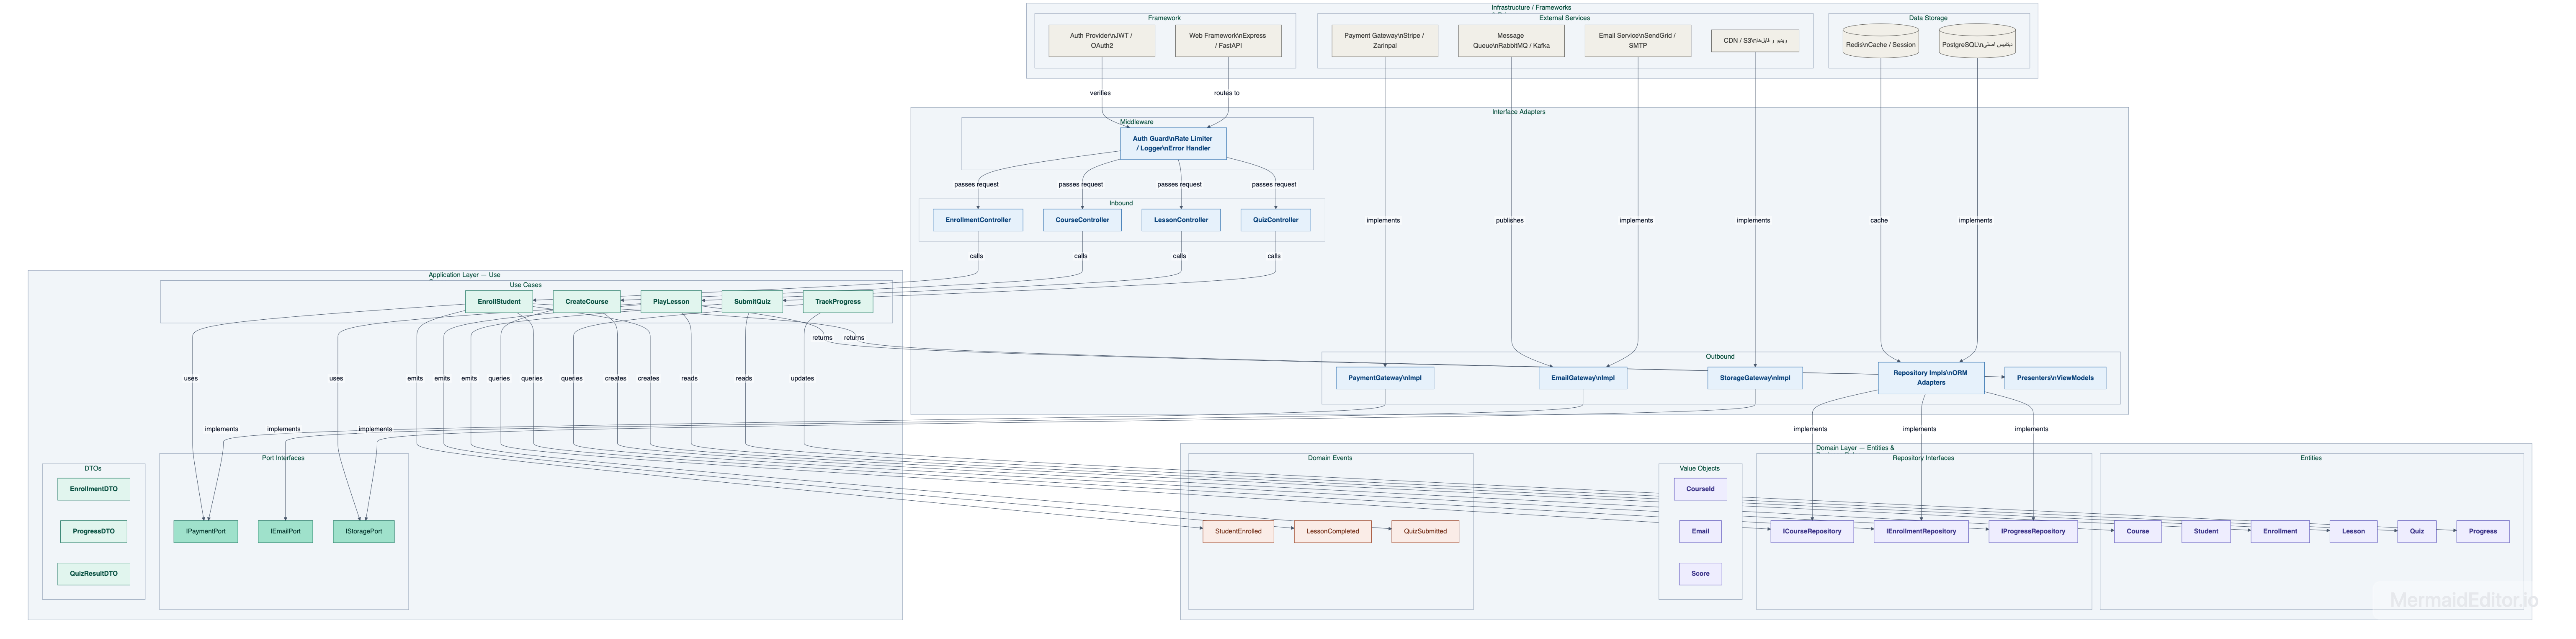
\includegraphics[width=1\textwidth]{1.png}
  \caption{معماری \lr{Clean Architecture} سامانه \lr{Courseware}}
\end{figure}

\subsubsection*{لایه Domain — هسته‌ی مرکزی}

این لایه هیچ وابستگی به هیچ کتابخانه‌ی خارجی ندارد و خالص‌ترین بخش سیستم است. اجزای آن عبارتند از:

\begin{itemize}
  \item \lr{Entities }: \lr{Course}، \lr{Lesson}، \lr{Student}، \lr{Enrollment}، \lr{Quiz}، \lr{Progress}
  \item \lr{Value Objects }: \lr{CourseId}، \lr{Email}، \lr{Score}، \lr{Duration}
  \item \lr{Domain Events }: \lr{StudentEnrolled}، \lr{LessonCompleted}، \lr{QuizSubmitted}
  \item \lr{Repository Interfaces }: قراردادهایی که لایه‌ی Infrastructure باید پیاده‌سازی کند
\end{itemize}

\subsubsection*{لایه Application — UseCases}

منطق تجاری اپلیکیشن را کنترل می‌کند و فقط به لایه‌ی Domain وابسته است.

\begin{table}[H]
    \centering
    \begin{tabular}{rl}
    \hline
    {مسئولیت} & {\lr{Use Case}} \\
    \hline
    اعتبارسنجی ثبت‌نام، پردازش پرداخت، ایجاد Enrollment & \lr{EnrollStudent} \\
    بررسی دسترسی، تولید URL امن محتوا، ثبت شروع مشاهده & \lr{PlayLesson} \\
    دریافت پاسخ‌ها، نمره‌دهی خودکار، ذخیره QuizResult & \lr{SubmitQuiz} \\
    محاسبه درصد پیشرفت، صدور گواهینامه در صورت تکمیل & \lr{TrackProgress} \\
    ایجاد دوره توسط مدرس، اعتبارسنجی محتوا & \lr{CreateCourse} \\
    \hline
    \end{tabular}
    \caption{UseCase های اصلی لایه‌ی Application}
    \end{table}

این لایه برای ارتباط با سرویس‌های خارجی فقط interface تعریف می‌کند. پیاده‌سازی واقعی در Infrastructure است.

\subsubsection*{لایه Adapters Interface}

داده را بین دنیای خارج و لایه‌ی Application تبدیل می‌کند.

\begin{itemize}
  \item {\lr{Controllers}}: \lr{HTTP request} را دریافت، اعتبارسنجی، و به \lr{DTO} تبدیل می‌کنند
  \item {\lr{Presenters}}: خروجی \lr{use case} را به فرمت \lr{JSON} مناسب برای کلاینت تبدیل می‌کنند
  \item {\lr{Repository Implementations}}: پیاده‌سازی واقعی \lr{interface} های \lr{Domain} با استفاده از \lr{ORM}
  \item {\lr{External Gateways}}: پیاده‌سازی \lr{Port Interface} ها 
  \item {\lr{Middleware}}: \lr{Auth Guard}، \lr{Rate Limiter}، \lr{Logger}، \lr{Error Handler}
\end{itemize}

\subsubsection*{لایه Infrastructure — Frameworks \& Drivers}

جزئیات فنی که قابل تعویض هستند و هیچ‌کدام به لایه‌های داخلی وابسته نیستند.

\begin{table}[H]
\centering
\begin{tabular}{rrl}
\hline
{بخش} & {توضیح} & {فناوری} \\
\hline
دیتابیس اصلی & ذخیره‌سازی دوره‌ها و ثبت‌نام‌ها & \lr{PostgreSQL} \\
Cache & کش query ها و session کاربران & \lr{Redis} \\
CDN / Storage & ویدیوها و فایل‌های درسی & \lr{AWS S3} \\
درگاه پرداخت & پردازش تراکنش‌های مالی & \lr{Zarinpal} \\
ارسال ایمیل & تأیید ثبت‌نام و یادآوری‌ها & \lr{SMTP} \\
Message Queue & رویدادهای async & \lr{RabbitMQ / Kafka} \\
فریم‌ورک وب & \lr{HTTP Server} & \lr{FastAPI} \\
\hline
\end{tabular}
\caption{اجزای لایه‌ی Infrastructure}
\end{table}

\subsubsection*{ماژول‌های اصلی سامانه}

\begin{table}[H]
    \centering
    \begin{tabular}{rl}
    \hline
    {مسئولیت} & {ماژول} \\
    \hline
    ایجاد، ویرایش، و انتشار دوره‌ها توسط مدرس & \lr{Course Management} \\
    ثبت‌نام دانش‌آموز، پرداخت، مدیریت دسترسی & \lr{Enrollment} \\
    پخش محتوا، ردیابی پیشرفت، مدیریت نشانک‌ها & \lr{Learning Engine} \\
    آزمون‌ها، تکالیف، نمره‌دهی، صدور گواهینامه & \lr{Assessment} \\
    احراز هویت، پروفایل، نقش‌ها & \lr{User Management} \\
    ایمیل، پوش نوتیفیکیشن، یادآوری ادامه‌ی درس & \lr{Notification} \\
    گزارش پیشرفت دانش‌آموزان و آمار دوره‌ها & \lr{Analytics} \\
    \hline
    \end{tabular}
    \caption{ماژول‌های اصلی سامانه‌ی Courseware}
    \end{table}

ماژول‌ها مستقیم به هم وابسته نیستند و از طریق \lr{Domain Events} ارتباط برقرار می‌کنند. وقتی \lr{StudentEnrolled} منتشر می‌شود، ماژول \lr{Notification} آن را دریافت و ایمیل می‌فرستد، بدون اینکه ماژول \lr{Enrollment} چیزی درباره‌ی \lr{Notification} بداند. این الگو \lr{Loose Coupling} را تضمین می‌کند و تعویض هر بخش را بدون تأثیر بر بقیه ممکن می‌سازد.